\documentclass[tikz,a4paper,12pt]{article}
\input{/home/pim/Desktop/huiswerk.tex}
\title{Game Theory 2019-2020: Lecture Notes}
\usepackage[english]{babel}
\usepackage{tikz}
\usetikzlibrary{graphdrawing.trees}

\author{Author: Pim Meulensteen\\
\href{mailto:pim.meulensteen@student.uva.nl}{Contact: pim.meulensteen@student.uva.nl}\\
\\
Course: Game Theory (6012B0460Y)\\
Lecturer: Prof. T.J.S. Offerman\\
}

\begin{document}
\maketitle
\tableofcontents
\clearpage

\pagestyle{headings}
\part{Lectures Notes}
\section{Introduction \& Perfect information}
Game theory is about strategically interdependent decision-making. In such situations the result of a decision also depends on the decisions of others. When making a decision people have to think about what others will do, who in turn are thinking about what others do and so on. Game theory offers several concepts and insights for understanding and analysing such situations and for making better strategic decisions

\begin{definition}[Game Theory]
      Game Theory studies mathematical models of strategic interaction (actions) among rational decision-makers (players).
\end{definition}


\begin{definition}[Normative Game Theory]
      Normative Game Theory is about improving real-world results of games.
\end{definition}


\begin{definition}[Postive Game Theory]
      Positive Game Theory is describing how people behave in real-world situations.
\end{definition}


\begin{definition}[(Non-)cooperative Game Theory]
      A game is cooperative if the players can form binding commitments externally enforced. Cooperative game theory focuses on predicting which coalitions will form, the actions that groups take and the resulting payoffs.

      Non-cooperative game theory , also know as competitive game theory, studies games with competition between individual players.
\end{definition}

\begin{definition}[Action]
      A set $A$ consisting of all the actions $a$ that, under some circumstances, are available to the decision-maker.
\end{definition}


\begin{definition}[Rational choice]
      An action chosen by a decision-maker is at least as good, according to her preferences, like every other available action.
\end{definition}


\begin{note}
      \normalfont  Within game Theory, we assume people can rank any two actions. However, this is not always the case. We are not always 100\% rational.
\end{note}

\begin{definition}[Payoff function]
      The payoff function $u : A \to \rr$ represents a decision-maker’s preferences if, for
      any actions $a, b \in A$
      $$u(a) > u(b) \iff \text{ the decision-maker prefers a to b}$$
\end{definition}

\begin{definition}[Strategic game]
      A strategic game - or normal form game - consists of three things:
      \begin{itemize}[nosep]
            \item a set of players $N$,
            \item for each player a set of actions $A$,
            \item for each player, (ordinal) preferences over the set of action profiles $u_i : A \to \rr$ for all $i \in N$.
      \end{itemize}
\end{definition}


\begin{example}[Prisoner's Dilemma]
      This game has two players. Each player has two actions: Fink or Quiet. The prisoners' dilemma has the action profiles with corresponding payoff:
      \begin{itemize}
            \item If Player 1 and Player 2 each betray the other, each of them serves two years in prison.
            \item If Player 1 betrays Player 2 but Player 2 remains silent, Player 1 will be set free and Player 2 will serve three years in prison (and vice versa)
            \item If Player 1 and Player 2 both remain silent, both of them will serve only one year in prison.
      \end{itemize}
      This can be visualized in the following payoff matrix:
      \begin{table}[h!]
            \begin{center}
                  \begin{tabular}{ c | c c }
                              & Quiet & Fink   \\ \hline
                        Quiet & $2,2$ & $0,3$  \\
                        Fink  & $3,0$ & $1, 1$
                  \end{tabular}
                  \vspace{-5pt}
                  \caption{Payoff matrix corresponding to the Prisoner's Dilemma.}
                  \vspace{-30pt}
            \end{center}
      \end{table}
\end{example}
\begin{theorem}
      Any function applied to the utility which does not change the oridinality\footnote{if $x > y$, then $f(x) > f(y)$}, will not change the game.
\end{theorem}


\begin{example}[Battle of the sexes]
      This game has two players: a wife and a husband. Each player has two actions: Bach or Stravinsky.
      The husband would prefer to go to Bach. The wife would rather go to Stravinsky. Both would prefer to go to the same place rather than different ones.
      This can be visualized in the following payoff matrix:
      \begin{table}[h!]
            \begin{center}
                  \begin{tabular}{ c | c c }
                                   & Bach  & Stravinsky \\ \hline
                        Bach       & $2,1$ & $0,0$      \\
                        Stravinsky & $0,0$ & $1, 2$
                  \end{tabular}
                  \vspace{-5pt}
                  \caption{Payoff matrix corresponding to the Battle of the sexes.}
                  \vspace{-30pt}
            \end{center}
      \end{table}
\end{example}


\begin{example}[Stag hunt]
      This game has two players: two identical hunters. Each hunter can individually choose to hunt a stag or hunt a hare. If an individual hunts a stag, they must have the cooperation of their partner to succeed. An individual can get a hare by himself, but a hare is worth less than a stag.
      This can be visualized in the following payoff matrix:
      \begin{table}[h!]
            \begin{center}
                  \begin{tabular}{ c | c c }
                             & Stag  & Hare   \\ \hline
                        Stag & $2,2$ & $0,1$  \\
                        Hare & $1,0$ & $1, 1$
                  \end{tabular}
                  \vspace{-10pt}
                  \caption{Payoff matrix corresponding to Stag Hunt.}
                  \vspace{-20pt}
            \end{center}
      \end{table}
\end{example}


\begin{definition}[Nash equilibrium]
      A Nash equilibrium is an action profile with the property that no player can do better given that other players adhere to their actions.
      \textit{Formally:} the action profile $a^*$ in a strategic game with ordinal preferences is a Nash
      equilibrium if, for every player $i$ and every action $a_i$ of player $i$, $a^*$ is at least as good
      according to player $i$'s preferences as the action profile $(a_i , a^*_{-i})$ in which $i$ chooses $a_i$
      while every other player $j$ chooses $a^*_j$.

      Or, for every player $i$
      \[
            u_i (a^*) > u_i(a_i , a^*_{-i} )
      \]
      for every action $a_i$ of player $i$ where $u_i$ represents player $i$'s preferences.
\end{definition}

\begin{definition}[Best Response]
      The Best Response for player $i$ is the set of player $i$'s best actions (denoted by $\mathcal{B}_i (a_{-i})$) when the list of the other
      players' actions is $a_{-i}$
      \textit{Formally}:
      \[
            \mathcal{B}_i (a_{-i}) = \{a_i \mid a_i \in A_i : u_i (a_i ,a_{-i} ) > u_i (a_i' ,a_{-i} )  \forall a_i' \in A_i\}
      \]
\end{definition}
\begin{corollary}
      In a Nash equilibrium every player plays best response to the other players' actions. \textit{Formally:}
      \[
            a^* \text{ is Nash equilibrium} \iff a^*_i \in \mathcal{B}_i (a^*_{-i} ) \forall i
      \]
\end{corollary}


\begin{definition}[Strictly dominating actions]
      We say a player $i$'s action $a_i''$ strictly dominates action $a_i'$ if
      \[u_i (a_i'' , a_{-i} ) > u_i (a_i' , a_{-i} )\]
      for every list of other players' actions $a_{-i}$. 
      
      This means that a player’s action strictly dominates another action if it 
      is superior, no matter what the other players do.
\end{definition}


\begin{definition}[Strictly dominated actions]
      If an action strictly dominates the action $a_i$, we say that $a_i$ is strictly dominated.
\end{definition}


\begin{corollary}
      \normalfont A strictly dominated action is not used in any Nash equilibrium.
\end{corollary}


\begin{definition}[Weakly Dominated actions]
      We say a player $i$'s action $a_i''$ strictly dominates action $a_i'$ if
      \[
            u_i (a_i'' , a_{-i} ) \ge u_i (a_i' , a_{-i} )
      \]
      for every list of other players' actions $a_{-i}$, and
      \[
            u_i (a_i'' , a_{-i} ) > u_i (a_i' , a_{-i} )
      \]
      for some list $a_{-i}$ of other players' actions.
\end{definition}


\begin{note}
      \normalfont A Weakly dominated action may be used in a Nash equilibrium.
\end{note}


\begin{example}
      Consider the following payoff matrix:
      \begin{table}[h!]
            \begin{center}
                  \begin{tabular}{ c | c c }
                              & Left  & Right  \\ \hline
                        Left  & $2,2$ & $0,3$  \\
                        Right & $3,0$ & $1, 1$
                  \end{tabular}
                  \caption{Payoff matrix corresponding to the Prisoner's Dilemma.}
            \end{center}
      \end{table}
      \vspace{-15pt}

      Row Player's action \textit{Bottom} is weakly dominated by \textit{Top}
      Column Player's action \textit{Right} is weakly dominated by \textit{Left}
      Nevertheless, there are two Nash equilibria: (\textit{Top}, \textit{Left}) and (\textit{Bottom}, \textit{Right}).
\end{example}


\begin{illustration}[Contributing to a public good]
      When building some public good (like street lights), there is a cost to that ($c_i$) and a value function ($v_i(c)$). Furthermore, each player has a maximum ($w_i$) they can contribute. This gives the following game:
      \begin{itemize}
            \item Players: two people.
            \item Actions: $0 < c_i < w_i$ .
            \item Preferences: $u_i (c_1 , c_2 ) = v_i (c_1 +c_2 ) - c_i$ for $i=1,2$.
      \end{itemize}

      Consider the perspective of player 1. 
      We assume $0 < \mathcal{B}_1(0) < w_1$ where $\mathcal{B}_1(0)$ is the best response when the other player contributes $0$.   
      Suppose that $u_1 (c_1 ,0)$ has an interior maximum thus $b_1(0)$ is player 1's best response to $c_ 2 = 0$;
      Now consider $\mathcal{B}_1(k)$, 1's best response to $c_2 = k$:
      \begin{align*}
            u_1(c_1 +k,0) & = v_1 (c_1 +k) - c_1 - k; \\
            u_1(c_1 ,k)   & = v_1 (c_1 +k) - c_1 ;
      \end{align*}
      Now it follows, by adding $k$ to both sides:
      \begin{align*}
            u_1(c_1 +k,0) + k & = v_1 (c_1 +k) - c_1 ; \\
            u_1(c_1 ,k)       & = v_1 (c_1 +k) - c_1 ;
      \end{align*}
      Therefore,
      \[
            u_1(c_1 ,k) =u_1(c_1 +k,0) + k;
      \]
      This means: for me to be indifferent to spend $c_1$ euros and player 2 spending $k$ euros or spending $c_1$ euros, player 2 spending $0$ and receiving $k$ euros.

      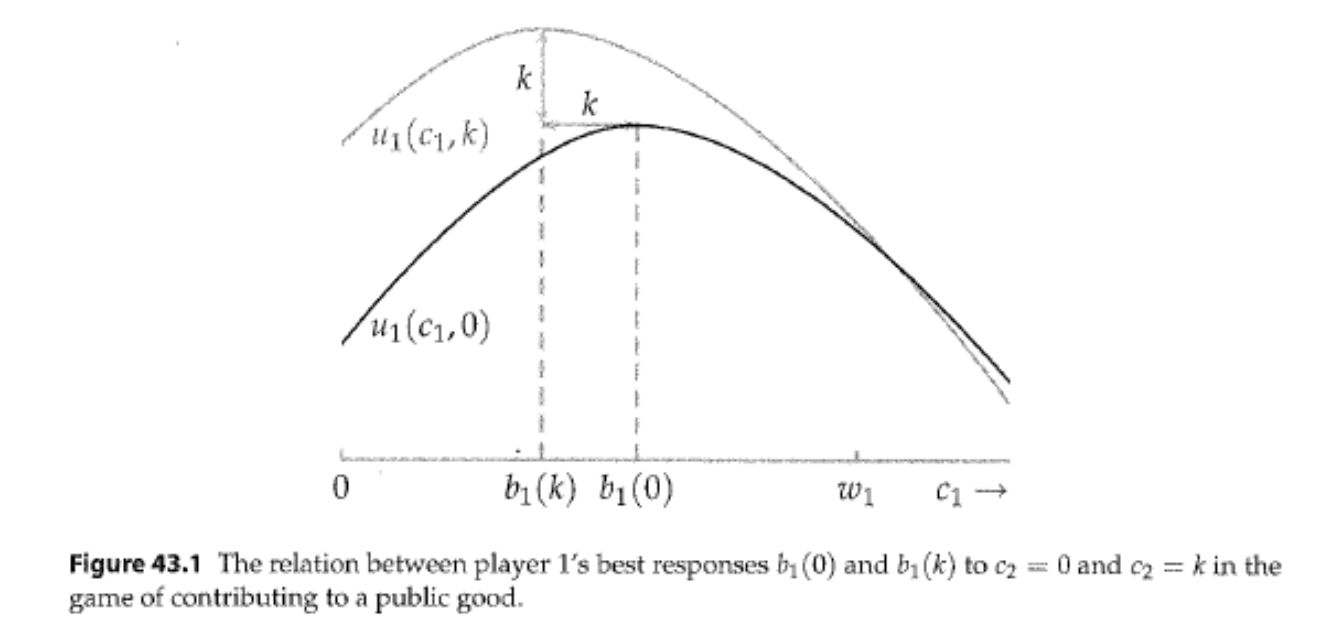
\includegraphics[width=1\textwidth]{im1.png}

      We now can say:
      if $k<b_1 (0)$ then $b_1(k)=b_1(0)- k$;
      if $k>b_1 (0)$ then $b_1( k)=0$;
      When doing a similar analysis applies to player 2: assume $b_1 (0) > b_2(0)$. Now we can say:
      if $k<b_2 (0)$ then $b_2(k)=b_2(0)- k$;
      if $k>b_2 (0)$ then $b_2(k)=0$;

      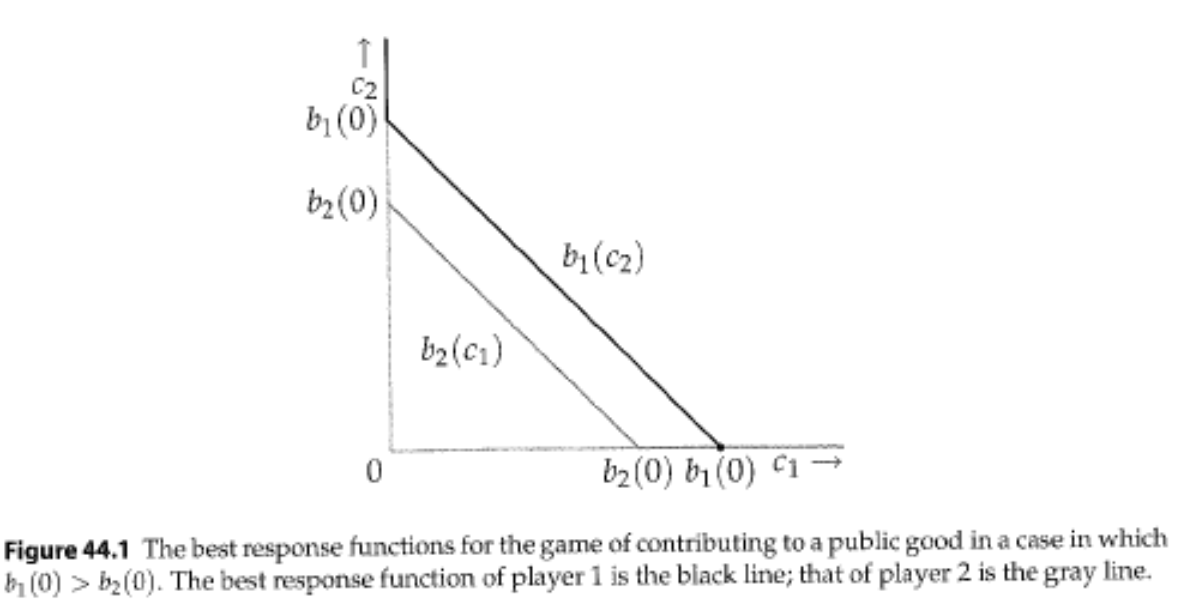
\includegraphics[width=1\textwidth]{im2.png}

      Since each player chooses best response, from the Graph it follows: $(b_1(0),0)$ is the Nash equilibrium if $b_1(0) > b_2(0)$. When $b_1(0) = b_2(0)$, the Nash equilibrium are all $(c_1,c_2) : c_1+c_2 = b_1(0) = b_2(0), c_1, c_2 \ge 0$. Lastly, when $b_1(0) < b_2(0)$,the Nash equilibrium is $(0,b_2(0))$.
\end{illustration}


\begin{definition}[Symmetric games]
      A strategic game with ordinal preferences is a \textbf{symmetric game} if the players' sets
      of actions are the same and the players' preferences are represented by $u_i$ with
      $u_i(a i , a_{-i} ) = u_j (a_j , a_{-j} )$ for all $i,j$.
\end{definition}


\begin{definition}[Symmetric Nash equilibrium]
      An action profile $a^*$ in a symmetric game is a \textbf{symmetric Nash equilibrium} if it is a Nash equilibrium and $a^*_i$ is the same for each player $i$.
\end{definition}
\clearpage

\section{Mixed strategy equilibrium}
\begin{definition}[Mixed strategy Nash equilibrium]
      The mixed strategy profile $\alpha^{*}$ is a \textbf{mixed strategy Nash equilibrium} of a strategic game with vNM preferences if for each player $i$ and every mixed strategy $\alpha_{i}$
      $$
            U_{i}(\alpha^*) \geq U_{i}\left(\alpha^*_{-i}, \alpha_{i}\right)
      $$
      holds.
\end{definition}


\begin{example}[Matching pennies]
      In the matching pennies game, each of two players flip a penny to heads or tails. The players then reveal their choices simultaneously. We have the following table corresponding to the payoff.
      \begin{table}[h!]
            \begin{center}
                  \begin{tabular}{ c | c c }
                             & Head    & Tail    \\ \hline
                        Head & $1,-1$  & $-1,1$  \\
                        Tail & $-1, 1$ & $1, -1$
                  \end{tabular}
                  \vspace{-5pt}
                  \caption{Payoff matrix for the Matching Pennis game}
                  \vspace{-20pt}
            \end{center}
      \end{table}
      Assume player 1 plays Head with probability $p$ (thus tail with probability $1-p$) and player 2 plays Head with probability $q$ (thus tail with probability $1-q$). Then:
      \[
            \ee_1[\pi(\text{head})]=q+(1-q)(-1)=2 q-1
      \]
      \[
            \ee_1[\pi(\text{tail})]=q(-1)+(1-q)=1-2 q
      \]
      Now, we can easily find the best response function for player one if player 2 is allowed to mix.
      \[
            \mathcal{B}_{1}(q)=\left\{\begin{array}{cl}
                  \{0\}                  & \text { if } q<\frac{1}{2} \\
                  \{p: 0 \leq p \leq 1\} & \text { if } q=\frac{1}{2} \\
                  \{1\}                  & \text { if } q>\frac{1}{2}
            \end{array}\right.
      \]

      \[
            \mathcal{B}_{2}(p)=\left\{\begin{aligned}
                  \{1\}                  & \text { if } p<\frac{1}{2} \\
                  \{q: 0 \leq q \leq 1\} & \text { if } p=\frac{1}{2} \\
                  \{0\}                  & \text { if } p>\frac{1}{2}
            \end{aligned}\right.\]
      When drawing these two functions, there is an intersection. This intersection is the Nash equilibrium. We can say:
      \[
            a^{*}: p =\frac{1}{2}; q = \frac{1}{2}
      \]
\end{example}


\begin{proposition}
      \label{2_important}
      A mixed strategy profile $\alpha^{*}$ in a strategic game with vNM preferences in which each player has finitely many actions is a mixed strategy Nash equilibrium\\
      $\iff$\\
      for each player $i$
      \begin{itemize}
            \item the expected payoff, given $\alpha_{-i}^*,$ to every action to which $\alpha_{i}^{*}$ assigns positive probability is the same;
            \item the expected payoff, given $\alpha_{-i}^{*},$ to every action to which $\alpha_{i}^{*}$ assigns zero probability is smaller than or equal to the expected payoff to any action to which $\alpha_{i}^{*}$ assigns positive probability.
      \end{itemize}
\end{proposition}


\begin{note}
      In simple terms, this means you are indifferent about the actions you are using and the actions that you are not using cannot give you a higher expected utility. This means you are choosing your best response. If every player chooses their best response, it is a Nash equilibrium.
\end{note}


\begin{corollary}
      Each player's expected payoff is in an  equilibrium is her expected payoff to any action that she uses with positive probability.
\end{corollary}


\begin{proof}
      Given a set of actions with positive probability for a player. If any action deviates from the other, either
      \begin{itemize}
            \item this action is a better option, and she should drop the other actions in this set.
            \item this action is a worse option, and she should drop this action from the set.
      \end{itemize}
      By induction, we can conclude that all expected payoffs are equal.
\end{proof}


\begin{proposition}
      Every strategic game with vNM preferences in which each player has finitely many actions has a mixed strategy equilibrium.
\end{proposition}
\begin{note}
      Note the use of `finite' here. There might be, but might not always be, a mixed strategy equilibrium in the case for infinite games. For example, the game where you choose the highest number. Here, there are infinite action with always a better option (choosing a higher number).
\end{note}


\begin{definition}[Dominated actions in strategic games with vNM preferences]
      Player $i$'s mixed strategy $\alpha_{i}$ strictly dominates action $\alpha$ if
      \[
            u_{i}(\alpha_{i}'', \alpha_{-i}) > u_{i}(\alpha_{i}', \alpha_{-i})
      \]
      for every list a of other players' actions.
\end{definition}


\begin{example}
      Consider the following game;:
      \begin{table}[h!]
            \begin{center}
                  \begin{tabular}{ c | c c c}
                              & $T_1$ & $T_2$ & $T_3$ \\ \hline
                        $S_1$ & $2,2$ & $0,3$ & $1,2$ \\
                        $S_2$ & $3,1$ & $1,0$ & $0,2$
                  \end{tabular}
            \end{center}
      \end{table}
      $T_1$ does not look like a good option. Claim: for player 2 the action profile $\alpha_2 = (0,q,1-1)$ is strictly better than than $T_1$. For this, there need to be
      \begin{itemize}
            \item For $S_1$: $3 \cdot q + 2(1-q) > 2 \iff q >0$
            \item For $S_2$: $0 \cdot q + 2(1-q) > 1 \iff q < \frac{1}{2}$
      \end{itemize}
      Now we can conclude our claim is true for $0 < q <
            \frac{1}{2}$. Thus $T_1$ is stricly dominated by $\alpha_2$ for some action profile (for example $(0,\frac{1}{3}, \frac{2}{3})$), and therefor not used in any mixed strategy Nash equilibrium.
      We can see in general when player 1 has profile $\alpha_1 = (0,\lambda, 1-\lambda)$, that
      \[
            U(T_1) = 2\cdot \lambda + 1 - \lambda = \lambda + 1 < \frac{7}{3}\lambda + \frac{4}{3}(1-\lambda) = \lambda + \frac{4}{3}\lambda = U(\alpha_2)s
      \]
\end{example}


\begin{illustration}[Volunteers dilema]
      We have the following game:
      \begin{itemize}
            \item Players: $n$ people witnessing a crime
            \item Each player $i$ chooses from \{call, don't call\};
            \item Preferences: vNM preferences
                  \begin{itemize}
                        \item $U$[nobody calls] $=0$
                        \item $U$[$i$ calls] $=v-c$
                        \item $U$[$i$ doesn't call, at least one other does] $= v$
                  \end{itemize}
      \end{itemize}
      
      This means calling costs $c$ and solving the crime gives $v$.
      \\
      Claim 1: this game has Nash equilibrium.
      One person calling is enough. Say one person calls, that person doesn't want to not call ($U$[nobody calls] $< U$[$i$ calls]). For the other persons, they don't want to call ($U$[$i$ calls] $< U$[$i$ doesn't call, at least one other does]). This means that the action profile where one player calls is a Nash equilibrium. This also means there are $n$ Nash equilibria: every player $i$ can call.\\
      \\
      Claim 2: there also is a symmetric Nash equilibrium (a Nash equilibrium where every player uses the same mixed strategy). This means every player is calls with the same probability $p$. We must be indifferent between these two actions (see Corollary \ref{2_important}).
      \begin{align*}
            EU[\text{call}]             & = EU[\text{not calling}]                                                          \\
            v-c                         & = 0\cdot P[\text{no one else calls}] + v\cdot P[\text{at least one player calls}] \\
            v-c                         & = v\cdot P[\text{at least one player calls}]                                      \\
            v-c                         & = v(1 - P[\text{no one player calls}])                                            \\
            v-c                         & = v - v\cdot P[\text{no one else calls}])                                         \\
            -c                          & = - v\cdot P[\text{no one else calls}]                                            \\
            P[\text{no one else calls}] & = \frac{c}{v}                                                                     \\
            (1-p)^{n-1}                 & = \frac{c}{v}                                                                     \\
            (1-p)                       & = (\frac{c}{v})^{\frac{1}{n-1}}                                                   \\
            p = 1 -(\frac{c}{v})^{\frac{1}{n-1}}
      \end{align*}

      \noindent Claim 3: when $n$ increases, $p$ decreases
\end{illustration}


\clearpage

\section{Extensive games with perfect information}
\begin{definition}
      Definition of extensive game with perfect information
      \begin{itemize}
            \item set of players
            \item set of terminal histories
            \item player function
            \item for each player, preferences terminal histories
      \end{itemize}
\end{definition}

\begin{example}[Mini-ultimatum game Proposer]
      We have two players: proposer and responder. Proposer stats with a choice: \textit{String} or \textit{Generous}. Then, the responder has the choice \textit{Accept} or \textit{Reject}. More formally, the specification of mini-ultimatum game is as follows:
      \begin{itemize}
            \item Players: proposer and responder
            \item Terminal histories:
                  (Stingy, Accept); (Stingy, Reject)
                  (Generous, Accept); (Generous, Reject)
            \item Player function:
                  \begin{itemize}
                        \item $P(\varnothing)=$ Proposer (Start of the game)
                        \item $P($Stingy$)=$ Responder
                        \item $P($Generous$)=$ Responder
                  \end{itemize}
            \item Preferences:
                  \begin{align*}
                        U_2(\text{Stingy},\text{Accept})=1    \\
                        U_1 (\text{Stingy},\text{Accept})=9   \\
                        U_2(\text{Stingy},\text{Reject})=0    \\
                        U_1 (\text{Stingy},\text{Reject})=0   \\
                        U_2(\text{Generous},\text{Accept})=5  \\
                        U_1 (\text{Generous},\text{Accept})=5 \\
                        U_2(\text{Generous},\text{Reject})=0  \\
                        U_1 (\text{Generous},\text{Reject})=0 \\
                  \end{align*}
      \end{itemize}
      This equal to the following tree:
      \tikzset{every picture/.style={line width=0.75pt}} %set default line width to 0.75pt        

      \begin{tikzpicture}[x=0.75pt,y=0.75pt,yscale=-1,xscale=1]
            %uncomment if require: 
            \path (0,300); %set diagram left start at 0, and has height of 300

            %Straight Lines [id:da20379485280914245] 
            \draw    (380,129) -- (444.49,193.49) ;
            \draw [shift={(445.9,194.9)}, rotate = 225] [color={rgb, 255:red, 0; green, 0; blue, 0 }  ][line width=0.75]    (10.93,-3.29) .. controls (6.95,-1.4) and (3.31,-0.3) .. (0,0) .. controls (3.31,0.3) and (6.95,1.4) .. (10.93,3.29)   ;
            %Straight Lines [id:da04579844714855119] 
            \draw    (380,129) -- (317.61,191.39) ;
            \draw [shift={(316.2,192.8)}, rotate = 315] [color={rgb, 255:red, 0; green, 0; blue, 0 }  ][line width=0.75]    (10.93,-3.29) .. controls (6.95,-1.4) and (3.31,-0.3) .. (0,0) .. controls (3.31,0.3) and (6.95,1.4) .. (10.93,3.29)   ;
            %Straight Lines [id:da01737775400298025] 
            \draw    (302,22) -- (380.39,100.39) ;
            \draw [shift={(381.8,101.8)}, rotate = 225] [color={rgb, 255:red, 0; green, 0; blue, 0 }  ][line width=0.75]    (10.93,-3.29) .. controls (6.95,-1.4) and (3.31,-0.3) .. (0,0) .. controls (3.31,0.3) and (6.95,1.4) .. (10.93,3.29)   ;
            %Straight Lines [id:da3603923805245839] 
            \draw    (302,22) -- (221.31,102.69) ;
            \draw [shift={(219.9,104.1)}, rotate = 315] [color={rgb, 255:red, 0; green, 0; blue, 0 }  ][line width=0.75]    (10.93,-3.29) .. controls (6.95,-1.4) and (3.31,-0.3) .. (0,0) .. controls (3.31,0.3) and (6.95,1.4) .. (10.93,3.29)   ;
            %Straight Lines [id:da15281111625407162] 
            \draw    (214,127) -- (278.49,191.49) ;
            \draw [shift={(279.9,192.9)}, rotate = 225] [color={rgb, 255:red, 0; green, 0; blue, 0 }  ][line width=0.75]    (10.93,-3.29) .. controls (6.95,-1.4) and (3.31,-0.3) .. (0,0) .. controls (3.31,0.3) and (6.95,1.4) .. (10.93,3.29)   ;
            %Straight Lines [id:da505919501748696] 
            \draw    (214,127) -- (151.61,189.39) ;
            \draw [shift={(150.2,190.8)}, rotate = 315] [color={rgb, 255:red, 0; green, 0; blue, 0 }  ][line width=0.75]    (10.93,-3.29) .. controls (6.95,-1.4) and (3.31,-0.3) .. (0,0) .. controls (3.31,0.3) and (6.95,1.4) .. (10.93,3.29)   ;

            % Text Node
            \draw (274,4) node [anchor=north west][inner sep=0.75pt]   [align=left] {Proposer};
            % Text Node
            \draw (380,126) node [anchor=south] [inner sep=0.75pt]   [align=left] {Responder};
            % Text Node
            \draw (346.1,157.9) node [anchor=south east] [inner sep=0.75pt]   [align=left] {\textit{Accept}};
            % Text Node
            \draw (414.95,158.95) node [anchor=south west] [inner sep=0.75pt]   [align=left] {\textit{Reject}};
            % Text Node
            \draw (316.2,195.8) node [anchor=north] [inner sep=0.75pt]   [align=left] {(5,5)};
            % Text Node
            \draw (445.9,197.9) node [anchor=north] [inner sep=0.75pt]   [align=left] {(0,0)};
            % Text Node
            \draw (214,124) node [anchor=south] [inner sep=0.75pt]   [align=left] {Responder};
            % Text Node
            \draw (180.1,155.9) node [anchor=south east] [inner sep=0.75pt]   [align=left] {\textit{Accept}};
            % Text Node
            \draw (248.95,156.95) node [anchor=south west] [inner sep=0.75pt]   [align=left] {\textit{Reject}};
            % Text Node
            \draw (150.2,193.8) node [anchor=north] [inner sep=0.75pt]   [align=left] {(9,1)};
            % Text Node
            \draw (279.9,195.9) node [anchor=north] [inner sep=0.75pt]   [align=left] {(0,0)};
            % Text Node
            \draw (258.95,60.05) node [anchor=south east] [inner sep=0.75pt]   [align=left] {\textit{Stingy}};
            % Text Node
            \draw (343.9,58.9) node [anchor=south west] [inner sep=0.75pt]   [align=left] {\textit{Generous}};
      \end{tikzpicture}

      Drawing a graph might be more intuitive, but not every game is discrete. For continuos games, working with formulas is easier (or sometimes the only possibility).
\end{example}

\begin{definition}[Strategy]
      A \textbf{strategy} of a player in an extensive game is a complete action plan. That is, it
      specifies an action for every situation where it is her turn to make a move.
\end{definition}

\begin{example}[Strategies in the mini-ultimatum game]
      In the mini-ultimatum game, the responder has 4 strategies

      \begin{enumerate}
            \item A A = Accept after Stingy, Accept after Generous
            \item A R = Accept after Stingy, Reject after Generous
            \item R A = Reject after Stingy, Accept after Generous
            \item R R = Reject after Stingy, Reject after Generous
      \end{enumerate}

      This extensive form game can be written in strategic form:
      \begin{table}[h!]
            \begin{center}
                  \begin{tabular}{ c | c c c c}
                                 & A A   & A R   & R A   & R R   \\ \hline
                        Stingy   & (9,1) & (9,1) & (0,0) & (0,0) \\
                        Generous & (5,5) & (0,0) & (5,5) & (0,0)
                  \end{tabular}
            \end{center}
      \end{table}
      pure strategy Nash equilibria:
      \begin{enumerate}
            \item (Stingy, A A)
            \item (Stingy, A R)
            \item (Generous, R A)
      \end{enumerate}
\end{example}


\begin{definition}[Nash equilibrium in an extensive game]
      The strategy profile $s^*$ in an extensive game with perfect information is a Nash
      equilibrium if, for every player $i$ and every strategy $r_i$ of player $i$:
      \[
            U_i (s^* ) > U_i (r_i , s_{-i}^* )
      \]
\end{definition}


\begin{definition}[Subgame]
      Let $\Gamma$ be an extensive game with perfect information. For any non-terminal
      history $h$ of $\Gamma$, the subgame $\Gamma(h)$ following the history h is the following extensive
      game.
      \begin{itemize}
            \item Players: players in $\Gamma$
            \item Terminal histories: set of sequences $h^{\prime}$ such that $(h, h^{\prime})$ is a terminal history of $\Gamma$
            \item Player function: $P(h,h^{\prime})$ is assigned to each subhistory $h^{\prime}$ of a terminal history
            \item Preferences: each player prefers $h^{\prime}$ to $h^{\prime \prime}$ if and only if she prefers $(h,h^{\prime})$ to $(h,h^{\prime \prime})$
      \end{itemize}
\end{definition}


\begin{example}[Subgames of the mini-ultimatum game Proposer]
      The mini-ultimatum game has three subgames:
      \begin{enumerate}
            \item The whole game
            \item The game after Stingy
            \item The game after Generous
      \end{enumerate}
\end{example}


\begin{definition}[Subgame prefect equilibrium]
      A subgame perfect equilibrium is a strategy profile $s^*$ with the property that in no
      subgame can any player $i$ do better by choosing a strategy different from $s_i^*$, given that
      every other player $j$ adheres to strategy $s_j^*$.
\end{definition}


\begin{corollary}
      From this definition, it follows:
      \begin{itemize}
            \item every subgame perfect equilibrium is a Nash equilibrium
            \item a subgame perfect equilibrium induces a Nash equilibrium in every subgame
            \item not every Nash equilibrium is subgame perfect
      \end{itemize}
\end{corollary}


\begin{example}[Subgame prefect equilibrium of the mini-ultimatum game]
      The mini-ultimatum game has three subgames:
      \begin{enumerate}
            \item (Stingy, A A) is a N.E. and subgame perfect
            \item (Stingy, A R) is a N.E. but not subgame perfect
            \item (Generous, R A) is a N.E. but not subgame perfect, this N.E. uses \textit{incredible threat}\footnote{The threat of choosing \textit{reject} when choosing \textit{stingy}, the \textit{proposer} wants to choose \textit{generous}. However, if the \textit{proposer} still chooses \textit{stingy}, the \textit{responder} will still \textit{accept}}
      \end{enumerate}
\end{example}


\begin{example}[Twist to the mini-ultimatum game]
      Let us define the utility function by $U_i(x,y) = x - \frac{1}{4} |x-y| $. Now, our table is

      \begin{table}[ht!]
            \begin{center}
                  \begin{tabular}{ c | c c c c}
                                 & A A    & A R    & R A   & R R   \\ \hline
                        Stingy   & (7,-1) & (7,-1) & (0,0) & (0,0) \\
                        Generous & (5,5)  & (0,0)  & (5,5) & (0,0)
                  \end{tabular}
            \end{center}
      \end{table}
      Now it is the case that unique subgame perfect equilibrium [Generous, Reject Accept].
\end{example}


\begin{illustration}[Stackelberg's model of duopoly]
      Cournot setting where firms move sequentially
      \[
            P_{d}(Q) = \left\{
            \begin{array}{ll}
                  (\alpha-Q) & \text { if } Q \leq \alpha \\
                  0          & \text { if } Q>\alpha
            \end{array}\right.
      \]

      \[
            C_{i}(q_{i})=\mathrm{cq}_{i}
      \]

      \begin{itemize}
            \item Players: 2 firms
            \item Terminal histories: set of all quantity pairs $(q_{1}, q_{2}), q_{1} \geq 0, q_{2} \geq 0$ $\cdot$
            \item Player function: $P(\emptyset)=1$ and $P\left(q_{1}\right)=2$ for all $q_{1}$
                  $\cdot$
            \item Preferences: $\pi_{i}=q_{i} P_{d}\left(q_{1}+q_{2}\right)-c_{i}\left(q_{i}\right)=\left\{\begin{array}{ll}q_{i}\left(\alpha-c-q_{1}-q_{2}\right) & \text { if } Q \leq \alpha \\ -c q_{i} & \text { if } Q>\alpha\end{array}\right.$
      \end{itemize}

      To find the Subgame perfect equilibrium, we use backward induction:

      First Order Condition: if $Q \leq \alpha,$ set $\frac{d\pi_2}{dq_2} = 0$ (+ check Second Order Condition )

      This implies $\frac{d\pi_2}{dq_2} q_{2}(\alpha-c-q_{1}-q_{2}) =  \alpha-c-q_{1}-q_{2}-q_{2}=0$, and thus $q_{2}=\frac{1}{2}(\alpha-c-q_{1})$.

      Thus
      \[
            \quad b_{2}\left(q_{1}\right)=
            \left\{\begin{array}{ll}
                  \frac{1}{2}(\alpha-c-q_{1}) & \text { if } q_{1} \leq \alpha-c \\
                  0                           & \text { if } q_{1}>\alpha-c
            \end{array}\right.
      \]
      This was the smallest subgame. Now, solve a bigger subgame. This is the whole game. Of course, player 1 anticipates player 2's response and maximizes
      \[\pi_{1}=q_{1}\left(\alpha-c-q_{1}-\left(\alpha-c-q_{1}\right) / 2\right)=q_{1}\left(\alpha-c-q_{1}\right) / 2\]
      Again, set $\frac{d\pi_1}{dq_1} = 0$ and calculate the derivative:
      \[0 = \frac{d\pi_1}{dq_1} q_{1}(\alpha-c-q_{1}-q_{2}) =
            \left(\alpha-c-q_{1}\right) / 2-q_{1} / 2
      \]
      \\
      \begin{tabular}{l|l|l}
            Subgame perfect outcome                  & Payoff                                   & Subgame perfect equilibrium                                        \\
            \hline $q_{1}^{*}=\frac{1}{2}(\alpha-c)$ & $\pi_{1}^{*}=\frac{1}{8}(\alpha-c)^{2}$  & $q_{1}^{*}=\frac{1}{2}(\alpha-c)$                                  \\
            $q_{2}^{*}=\frac{1}{4}(\alpha-c)$        & $\pi_{2}^{*}=\frac{1}{16}(\alpha-c)^{2}$ & $b_{2}\left(q_{1}\right)=\left\{\begin{array}{cc}
                        \frac{1}{2}(\alpha-c-q_{1}) & \text { if } q_{1} \leq \alpha-c
                        \\ 0 & \text { if } q_{1}>\alpha-c\end{array}\right.$
      \end{tabular}

      Now, firm 1 is more aggressive and earns higher profit than in Cournot duopoly $[\frac{1}{9}(\alpha-c)^{2} ]$
\end{illustration}


\clearpage

\section{Bayesian games}
\begin{definition}[Bayseian Game]
      A \textbf{Bayesian game} is a game in which players have incomplete information about the other players. 
      A player may not know the exact payoff functions of the other players, but instead have beliefs about these payoff functions. 
      These beliefs are represented by a probability distribution over the possible payoff functions.
\end{definition}


\begin{example}[Battle of Sexes]
      Let us start with an example using the Battle of the Sexes game. We assume:
      \begin{itemize}
            \item player 1 does not know player 2's preference
            \item player 2 knows player 1's preference
      \end{itemize}
      This means there are two cases: \textit{player 2 wants to meet} or \textit{player 2 does not want to meet}. The case of \textit{player 2 wants to meet} is the standard Battle of the Sexes game. Player 2 will have payoff 0 if they meet, and keep her preference for S over B.

      \begin{table}[h!]
            \begin{center}
                  \begin{tabular}{ c | c c c c}
                          & B     & S     & \\ \hline
                        B & (2,1) & (0,0)   \\
                        S & (0,0) & (1,2)
                  \end{tabular}
                  \vspace{-5pt}
                  \caption{Situation where player 2 wants to meet}
                  \vspace{-25pt}
            \end{center}
      \end{table}

      \begin{table}[h!]
            \begin{center}
                  \begin{tabular}{ c | c c c c}
                          & B     & S     & \\ \hline
                        B & (2,0) & (0,2)   \\
                        S & (0,1) & (1,0)
                  \end{tabular}
                  \vspace{-5pt}
                  \caption{Situation where player 2 does not want to meet}
                  \vspace{-25pt}
            \end{center}
      \end{table}
\end{example}


\begin{example}[Nash Equiliberum in Battle of Sexes]
      Let us give both situations a chance: $p_{m(eet)} = p_{a(void)} = 0.5$.
      Only player 2 can choose, since she knows player 1's preference.
      However, player 1 does not know about player 2's preference.
      We can still make table for the player 1's expected payoff.
      Here $(A,B)$ is choice $A$ when not meeting and $B$ when meeting.

      \begin{table}[h!]
            \begin{center}
                  \begin{tabular}{ c | c c c c}
                          & (B,B) & (B,S) & (S,B) & (S,S) \\ \hline
                        B & 2     & 1     & 1     & 0     \\
                        S & 0     & 0.5   & 0.5   & 1
                  \end{tabular}
                  \vspace{-5pt}
                  \caption{Expected payoffs for player 1.}
                  \vspace{-25pt}
                  \label{table:payoff1}
            \end{center}

      \end{table}

      From this table, we can read that the best response for player 1 is $B$.
      When player 1 chooses $B$, player two would want to pick $B$ (payoff 1) with $p_{m} = 0.5$ and S (payoff 2) with $p_{a} = 0.5$.
      This means $\mathcal B_2 (B) = (B,S)$. This means $(B,(B,S)$ is a Nash Equilibrium of this game.

      When player 1 chooses $S$, player two would want to pick $S$ (payoff 2) with $p_{m} = 0.5$ and $B$ (payoff 1) with $p_{a} = 0.5$.
      However, player 1 would prefer $B$. This means $(S,(S,B)$ is not a Nash Equilibrium of this game.
      In formulae: $\mathcal B_2(S) = (S,B)$ but $\mathcal B_1(S,B) = B \implies$ player 1 will not choose $S$.
\end{example}


\begin{definition}[Formal Bayesian Game]
      A \textbf{Bayesian Game} has
      \begin{itemize}
            \item players: a set $N$
            \item states: a set  $\omega$
            \item actions: a set $A$
            \item signals: a function $\tau : \omega \to S$ where $S$ is a belief of states of the world.
            \item Bernoulli payoff function over $(a, \omega )$
      \end{itemize}
\end{definition}


\begin{example}[Battle of Sexes as a Bayesian Game]
      We can give the Battle of Sexes as a Bayesian Game as follows:
      \begin{itemize}
            \item players $N = \{\text{player 1, player 2}\}$
            \item states $\omega = \{\text { meet, avoid }\}$
            \item actions $a = \{ B , S \}$ for each player
            \item signals
                  \begin{itemize}
                        \item (uninformed) player 1: $\tau(\text {meet})=\tau(\text {avoid})=z$
                        \item (informed) player 2: $\tau(\text {meet})=m ; \tau(\text {avoid})=v$
                  \end{itemize}
            \item given signal, belief about states
                  \begin{itemize}
                        \item player 1 assigns prob. $1 / 2$ to either state after $z$
                        \item player 2 assigns prob. 1 to meet after $m$
                        \item player 2 assigns prob. 1 to avoid after $v$
                  \end{itemize}
            \item Bernoulli payoff function over $(a, \omega)$, best viewed in Table \ref{table:payoff1}
      \end{itemize}
\end{example}


\begin{example}[Battle of Sexes with both players uncertain]
      This game is like the example above, but now player 1 is also uncertain.
      Let $y$ be `wants to meet' and $n$ be `does not want to meet'.
      Let $ab$ be player 1 wants action $a$ and player 2 wants action $b$.
      Players only know their own state. We give $y_i$ and $y_i$ to players $i \in \{1,2\}$

      \begin{itemize}
            \item player 1's belief: player 2 wants to meet with probability 1/2
            \item player 2's belief: player 1 wants to meet with probability 2/3
            \item player 1 receives signals $y_1$ in $yy$ or $yn$, $n_1$ in $ny$ or $nn$
            \item player 2 receives signals $y_2$ in $yy$ or $ny$, $n_2$ in $yn$ or $nn$
      \end{itemize}
      This gives:
      \begin{itemize}
            \item Type $y_1$ believes $pr[yy]=pr[yn]=1/2$
            \item Type $y_2$ believes $pr[yy]=2/3$; $pr[ny]=1/3$
      \end{itemize}
      Claim: ((B,B), (B,S)) N.E.; ((S,B), (S,S)) N.E.
      \begin{proof}
            We first proof two lemmas.
            \begin{enumerate}[label=Lemma \arabic*.]
                  \item $\mathcal B_1 (B,S) = (B,B)$\\
                        We have two cases $y_1$ and $n_1$, which both have two cases $B$ and $S$.
                        \begin{enumerate}[label=(\roman*)]
                              \item type $y_1$ of player 1
                                    \begin{itemize}
                                          \item $\pi_{y_1} (B,(B,S)) = (1/2)\cdot 2+(1/2)\cdot 0 = 1$
                                          \item $\pi_{y_1} (S,(B,S)) = (1/2)\cdot 0+(1/2)\cdot 1 = 1/2$
                                    \end{itemize}
                              \item type $n_1$ of player 1
                                    \begin{itemize}
                                          \item $\pi_{n_1} (B,(B,S)) = (1/2)\cdot 0+(1/2)\cdot 2 = 1$
                                          \item $\pi_{n_1} (S,(B,S)) = (1/2)\cdot 1+(1/2)\cdot 0 = 1/2$
                                    \end{itemize}
                        \end{enumerate}

                  \item $\mathcal B_2 (B,B) = (B,S)$\\
                        We have two cases $y_2$ and $n_2$, which both have two cases $B$ and $S$.
                        \begin{enumerate}[label=(\roman*)]
                              \item type $y_2$ of player 2
                                    \begin{itemize}
                                          \item $\pi_{y_2} ((B,B),B) = (2/3)\cdot 1+(1/3)\cdot 1 = 1$
                                          \item $\pi_{y_2}((B,B),S) = (2/3)\cdot 0+(1/3)\cdot 0 = 0$
                                    \end{itemize}
                              \item type $n_2$ of player 2
                                    \begin{itemize}
                                          \item $\pi_{n_2}((B,B),B) = (2/3)\cdot 0+(1/3)\cdot 0 = 0$
                                          \item $\pi_{n_2} ((B,B),S) = (2/3)\cdot 2+(1/3)\cdot 2 = 2$
                                    \end{itemize}
                        \end{enumerate}
            \end{enumerate}
            By Lemma 1, 2 we can conclude $((B,B), (B,S))$ is a Nash equilibrium. 
            The proof for $((S,B), (S,S))$ is similar and left as an exercise for the reader.
      \end{proof}
\end{example}


\begin{example}
      We can give the Battle of Sexes with two uncertain players as a Bayesian Game as follows:
      \begin{itemize}
            \item players $N = \{\text{ player 1, player 2}\}$
            \item states $\omega = \{\text { yy,yn,ny,nn}\}$
            \item actions $a = \{ B , S \}$ for each player
            \item signals
                  \begin{itemize}
                        \item  player $1$:
                              \begin{itemize}
                                    \item $\tau_1(yy) = \tau_1(yn) = y_1$
                                    \item $\tau_1(ny) = \tau_1(nn) = n_1$
                              \end{itemize}
                        \item  player $2$:
                              \begin{itemize}
                                    \item $\tau_2(nn) = \tau_2(yn) = n_2$
                                    \item $\tau_2(ny) = \tau_2(yy) = y_2$
                              \end{itemize}
                  \end{itemize}
            \item given signal, belief about states
                  \begin{itemize}
                        \item player 1 assigns prob. 1/2 to each state $yy$ and $yn$ after $y 1 $
                        \item player 1 assigns prob. 1/2 to each state $ny$ and $nn$ after $n 1 $
                        \item player 2 assigns prob. 2/3 to $yy$ and 1/3 to $ny$ after $y 2 $
                        \item player 2 assigns prob. 2/3 to $yn$ and 1/3 to $nn$ after $n 2$
                  \end{itemize},
            \item Bernoulli payoff function over $(a, \omega)$, best viewed in a table from the (old) lecture notes.
      \end{itemize}
\end{example}


\begin{definition}[Nash equilibrium of a Bayesian game]
      A \textbf{Nash equilibrium of a Bayesian game} is a Nash equilibrium of the strategic game
      (with vNM preferences) defined as follows:
      \begin{itemize}
            \item \textit{Players}: set of all pairs $(i,t_i)$ in which i is the player and $t_i$ is one of the signals that i may receive
            \item \textit{Actions}: set of actions of each player $(i,t_i)$ is the set of actions of i in Bayesian game
            \item \textit{Preferences}: a Bernoulli payoff function of $(i,t_i)$ such that
                  \[
                        \pi_{i} [a_{i}, t_{i}] = \sum_{\omega \varepsilon \Omega} \operatorname{Pr}\left(\omega \mid t_{i}\right) u_{i}\left[\left\{a_{i}, a_{-i}^{+}(\omega)\right\}, \omega\right]
                  \]
                  where
                  \[
                        a^{+}(\omega) = a_j(\tau_j(\omega))
                  \]
      \end{itemize}
\end{definition}


\begin{example}[Public good II]
      Public good is provided if and only if at least one player contributes (at known cost $c$)
      Each individual is privately informed about $v_i$ , draw from $F(v)$, $0 < v_min < c < v_max$
\end{example}


\begin{example}[Bayesian game for Public good II] 
      The Public good II can be modelled as:
      \begin{itemize}
            \item Players: $n$ individuals
            \item States: set of all profiles $(v_1 , \ldots , v_n )$
            \item Actions: each player chooses $0$ or $c$
            \item Signals: $τ_i (v_1 ,\ldots, v_n ) = v_i$
            \item Beliefs: player $i$ assigns probability $F(v_1 ) F(v_2 )\ldots F(v_{i-1} ) F(v_{i+1} )\ldots F(v_n )$ to the event that the valuation of every other player $j$ is at most $v_j$
            \item Preferences of player $i$:
                  \begin{itemize}
                        \item $\pi_i =0$ if no one contributes
                        \item $\pi_i =v_i$ if $i$ does not contribute and at least one other does
                        \item $\pi_i =v_i - c$ if $i$ contributes
                  \end{itemize}
      \end{itemize}
\end{example}


\begin{example}[Symmetric Nash Equilibrium of Public good II]
      An example of a symmetric action profile is: $0$ for all $i$. 
      This is symmetric, but not a Nash Equilibrium. 
      I would rather spend $c$ to receive $v_i - c$. 
      Another such option is $c$ for all $i$. 
      But then, deviating to $0$ will increase my payoff from $v_i - c$ to $v_i$. 
      Thus, this is also not a Nash Equilibrium. 
      A candidate for such a Nash Equilibrium is: $c$ if $c \ge v^{*}$.

      If a player $i$ draws $v^{*}$, she is indifferent about playing $c$ or $0$. To prove this, we look at the expected utility. This is
      \[
            \mathbb{E}_i(\{c\} \mid v_i, s_{-1}) = v_i -c
      \]
      and
      \begin{align*}
            \mathbb{E}_i(\{0\} \mid v_i, s_{-1}) & = 0\cdot\mathbb{P}(\text{others do not contribute}) + v_i \cdot \mathbb{P}(\text{at least one other contributes})
            \\&=
            0 + v_i(1 - \mathbb{P}(\text{others do not contribute})) \tag{Note: $F(v^{*}) =\pp (v < v^{*}$}
            \\&=
            v_i(1 - F(v^{*})^{n-1})
      \end{align*}
      Player $i$ which $v_i = v^{*}$ will be indifferent if $\mathbb{E}_i(\{c\} \mid v_i, s_{-1}) = \mathbb{E}_i(\{0\} \mid v_i, s_{-1})$. This gives
      \begin{align*}
            v^{*} -c & = v^{*}(1 - F(v^{*})^{n-1})
            \\
            v^{*} -c & = v^{*} - v^{*}F(v^{*})^{n-1})
            \\
            c        & = v^{*}F(v^{*})^{n-1})
      \end{align*}
      If $v_i < v^{*}$, then $v_iF(v^{*})^{n-1} <  v^{*} F(v^{*})^{n-1} = c$. Then $-v_iF(v^{*})^{n-1}  > -c$. Now $v_i-v_iF(v^{*})^{n-1}  > v_i-c$ which is equal to $\mathbb{E}_i(\{0\} \mid v_i, s_{-1}) > \mathbb{E}_i(\{c\} \mid v_i, s_{-1})$. Thus, if $v_i < v^{*}$ then $i$ would want to not contribute.

      If $v_i > v^{*}$, then $v_iF(v^{*})^{n-1} >  v^{*} F(v^{*})^{n-1} = c$. Then $-v_iF(v^{*})^{n-1}  < -c$. Now $v_i-v_iF(v^{*})^{n-1}  < v_i-c$ which is equal to $\mathbb{E}_i(\{0\} \mid v_i, s_{-1}) < \mathbb{E}_i(\{c\} \mid v_i, s_{-1})$. Thus, if $v_i > v^{*}$ then $i$ would want to contribute.

      Now, we have identified the strategy `$c$ if $v_i > v^{*}$' as an equilibrium.
\end{example}


\begin{remark}
      In this example, the equilibrium is not in the best interest of the public good.
\end{remark}
\clearpage

\section{Extensive games with imperfect information}
\begin{definition}[Inforamtion Set]
    An \textbf{information set} is a collection of histories with the the property that the player who is going to move, doesn't know which history has been reached given that one of these histories was reached.
\end{definition}


\begin{definition}[information Partition]
    An \textbf{information partition} is a collection of information sets.
\end{definition}


\begin{example}
    Assume that after player $i$ moves $H_i = \{C,D,E\}$
    \begin{enumerate}[label=P\arabic*:]
        \item $\{C\}, \{D,E\}$: player knows whether C occurred or not
        \item $\{C\}, \{D\}, \{E\}$: player knows whether C, D or E occurred
        \item $\{C,D,E\}$: player does not know whether C, D or E occurred
    \end{enumerate}
\end{example}

\begin{remark}
    Any strategic game can be presented as an extensive game with imperfect information.
\end{remark}

\begin{example}[Battle of Sexes]
    In the Battle of Sexes, player 2 does not know wether she is on the left or right side of the tree. This is denoted by the red line with `2'. In any information set, it must be the case that the player is choosing between the same actions. If this is not the case, the property (unknown history) from an information set is not longer true.

    \begin{tikzpicture}[->]
        \node {Start}
        child { node {B}
                child { node {B} child {node{(2,1)}}}
                child { node {S} child {node{(0,0)}}}
            }
        child[color=white] { node[color=red,] {--------1--------} child {node[color=red] {---2---}}}
        child { node {S}
                child { node {B} child {node{(0,0)}}}
                child { node {S} child {node{(1,2)}}}
            };
    \end{tikzpicture}
\end{example}


\begin{illustration}[Definition extensive game/application to BoS]Formally, a extensive game has the following form:
    \begin{itemize}[noitemsep]
        \item Players
              \begin{itemize}[noitemsep]
                  \item Player 1
                  \item Player 2
              \end{itemize}
        \item Terminal histories
              \begin{itemize}[noitemsep]
                  \item (B,B)
                  \item (B,S)
                  \item (S,B)
                  \item(S,S)
              \end{itemize}
        \item Player function
              \begin{itemize}[noitemsep]
                  \item $P(\varnothing)=1$
                  \item $P(B)=2$
                  \item $P(S)=2$
              \end{itemize}
        \item Chance moves: none
        \item Information partitions:
              \begin{itemize}[noitemsep]
                  \item Player 1: $\varnothing$
                  \item Player 2: $\{B,S\}$
              \end{itemize}
        \item Preferences: as given in the graph above.
    \end{itemize}
\end{illustration}

\begin{illustration}[Card game] Our Card game is played as follows:
    \begin{itemize}
        \item Player 1 and player 2 put \$1 in the pot.
        \item A card is drawn.
        \item Player 1 is informed whether card is `high' or `low', player 2 is not informed.
        \item Player 1 can choose between (`see' and `raise')
              \begin{itemize}
                  \item If Player 1 chooses `see', then the game is finished. The card determines who wins dollar. `high' means player 1 gets the money, `low' means player 2 gets the money.
                  \item If player 1 chooses `raise', then she adds \$1 to the pot. Then Player 2 can choose (`pass' or `meet')
                        \begin{itemize}
                            \item If player 2 chooses `pass', player 1 takes the money.
                            \item If player 2 chooses `meet', she adds \$1 to pot.
                        \end{itemize}
              \end{itemize}
    \end{itemize}
\end{illustration}


\begin{illustration}[Nash Equilibrium of Card game] To find the Nash Equilibrium of the Card Game, write down the game in strategic form. In this table, (Raise, See) denotes player 1’s strategy to Raise after High and See after Low.

    \begin{table}[h!]
        \begin{center}
            \begin{tabular}{ c | c c c c}
                             & Pass   & Meet                           & \\ \hline
                Raise, Raise & (1,-1) & (0,0)                            \\
                Raise, See   & (0,0)  & ($\frac{1}{2}$,$-\frac{1}{2}$)   \\
                See, Raise   & (1,-1) & ($-\frac{1}{2}$,$\frac{1}{2}$)   \\
                Raise, Raise & (0,0)  & (0,0)
            \end{tabular}
            \caption{Strategic form of Card game}
        \end{center}
    \end{table}
    We can conclude that there are no pure strategies Nash equilibrium. Furthermore, (See, See) is strictly dominated by ($\frac{1}{2}$, Raise Raise; $\frac{1}{2}$, Raise See). This means (See, See) is not played in any Nash equilibrium.
    We also see that (See, Raise) is weakly dominated by (Raise, Raise). Given that $q=1$ (probability 1 to pass) cannot be part of Nash equilibrium, (See, Raise) is not used in any Nash equilibrium. We can now reduce our table.

    \begin{table}[h!]
        \begin{center}
            \begin{tabular}{ c c c c c}
                           & Pass   & Meet                           &      \\ \hline
                Raise, See & (0,0)  & ($\frac{1}{2}$,$-\frac{1}{2}$) & p    \\
                See, Raise & (1,-1) & ($-\frac{1}{2}$,$\frac{1}{2}$) & 1 -p \\
                           & q      & 1-q
            \end{tabular}
            \caption{Reduced Strategic form of Card game with probabilities}
        \end{center}
    \end{table}

    There are mixed strategies Nash equilibria in the remaining game. We have row-player indifferent if $q = (1/2)(1-q)$, thus $q = 1/3$. We also have column-player indifferent if: $-p = -(1/2)(1-p)$, thus $p = 1/3$.

    So, unique Nash equilibrium:
    player 1 assigns 1/3 to (Raise, Raise); 2/3 to (Raise, See) and
    player 2 assigns 1/3 to pass; 2/3 to meet

    In words, this means player 1 will always chooses `raise' after `high' and bluffs after `low' with probability 1/3

    This means that Card Game is favorable to player 1. You should refuse the role of player 2 if you can.
\end{illustration}


\begin{illustration}[Repated games: prisoner's dilemma] The main idea of this game is to sustain cooperation in equilibrium by threatening to switch to punishment if the other does not cooperate.

    \begin{table}[h!]
        \begin{center}
            \begin{tabular}{ c | c c c c}
                  & C     & D     & \\ \hline
                C & (2,2) & (0,3)   \\
                D & (3,0) & (1,1)
            \end{tabular}
            \caption{Payoff matrix for the prisoner's dilemma}
        \end{center}
    \end{table}

    There are two strategies:\\
    \textbf{Grim trigger strategy}
    \begin{itemize}
        \item start with C
        \item continue with C as long as other player chooses C
        \item if in any period other chooses D, then choose D in every subsequent period
    \end{itemize}
    \textbf{Tit-for-tat}
    \begin{itemize}
        \item start with C
        \item do whatever the other player did in previous period
    \end{itemize}
    We have some notation. Player $i$ uses discount factor $\delta$ for which $0 < \delta < 1$
    $$
        u_i(a^{1}, a^{2}, \ldots, a^{{T}}) = u_i(a^{1})+\delta u_i(a^{2})+\delta^{2} u_i(a^{3})+\ldots+\delta^{{T}-1} u_i(a^{{T}})
        =\sum_{t=1}^{T} \delta^{t-1} u_i(a^{t})
    $$
    There is a possibility that $T \to \infty$. Or that there is a $p$: a probability the game is finished at a given period.
\end{illustration}

\begin{example}
    Let $c$ be the value that makes player indifferent between payoffs $c, c, c, ... $ and payoffs
    $w^1 , w^2 , w^3 , ...$.
    Let $V$ denote the value of discounted sum $w^1 , w^2 , w^3 , ...$. We can find this $c$ as follows:
    \begin{align*}
        V =           & c + c\delta + c\delta^2 + c\delta^3 + ... \\
        V\delta =     & c\delta + c\delta^2 + c\delta^3 + ...     \\
        V-\delta V =  & c \tag{subtract \delta V from both sides} \\
        (1-\delta)V = & c
    \end{align*}
    So discounted average $c$ equals $(1 - \delta)V$
\end{example}

\begin{remark}
    A repeated game is an extensive game with perfect information and
    simultaneous moves. This mean we can use concept of subgame perfection. If the game is finitely repeated $n$ times, we can apply backwards induction (starting at the $n$th period).
\end{remark}

\begin{example}[Finitely repeated Prisoner's dilemma]
    Unique subgame perfect equilibrium: each player's strategy chooses D in every period (proof by backward induction). In any finitely repeated game every Nash equilibrium generates outcome (D,D) in every period. To support cooperation in equilibrium, it is required that the game is infinitely repeated.
\end{example}


\begin{illustration}
    Some Nash equilibria of infinitely repeated PD
    \begin{enumerate}

        \item Every player always plays D whatever happened
        \item Grim trigger strategy is N.E. if $\delta$ is sufficiently large. Assume other player plays grim trigger and that layer $i$ considers to deviate to D in period k. The discounted average deviation from period $k$ equals
              $(1-\delta)(3+\delta+\delta 2 +\delta 3 +...)=(1-\delta)(3+\delta/(1-\delta))=3(1-\delta)+ \delta$
              discounted average if $i$ sticks to grim trigger $ = 2$
              In conclusion, Grim trigger is a best response if
              $$2 > 3(1-\delta)+ \delta \iff \delta > 1/2$$
        \item  Tit-for-tat
              Assume other player plays tit-for-tat
              and that player $i$ considers to deviate to D in period $k$
              \begin{enumerate}


                  \item Player $i$ reverts to $C$ in period $k+1$. If this is part of her best response, she should continue alternating (situation is stationary). The discounted average payoff alternating from period $k$:
                        \[(1-\delta)(3+0\delta+3\delta 2 +0\delta 3 +3\delta 4 +...)=3(1-\delta)/(1-\delta 2 )=3/(1+\delta)
                        \]
                        Alternating does not beat tit-for-tat if
                        \[
                            3/(1+\delta) < 2 \iff \delta > 1/2
                        \]

                  \item player $i$ sticks to D after $k$. Then she earns
                        $$(1-\delta)(3+\delta+\delta 2 +\delta 3 +...=(1-\delta)(3+\delta/(1-\delta))=
                            3(1-\delta)+ \delta \le 2 \iff \delta \ge 1/2$$
              \end{enumerate}
    \end{enumerate}

    But many more outcomes can be supported in equilibrium of the infinitely repeated prisoner's dilemma.
\end{illustration}

\begin{theorem}[Folk Theorem]
    \begin{itemize}
        \item For any discount factor $\delta$ with $0<\delta<1$, the discounted average payoff of any player $i$ in any Nash equilibrium is at least $u_i (D,D)$.
        \item Let $(x_1 ,x_2)$ be a feasible pair of payoffs such that $x_i >u_i (D,D)$ for each $i$. There exists a
              $\delta^* \le 1$ such that if $\delta>\delta^* $, then the game has a N.E. in which the discounted payoff of each
              player $i$ is $x i$ .
        \item For any $\delta$ the game has a N.E. in which the average discounted payoff of player $i$ equals $u_i (D,D)$
    \end{itemize}
\end{theorem}
\begin{proof}

\end{proof}
\begin{illustration}[Nash equilibria of infinitely repeated PD with mistakes]
    What about environments where players may make mistakes? grim trigger does not do so well, tit-for-tat works better. But, the winner is Pavlov strategy
    ("win-stay lose-change"):
    \begin{itemize}
        \item Start with C
        \item Choose C if previous outcome was (C,C) or (D,D)
        \item Choose D after any other history
    \end{itemize}
\end{illustration}


\clearpage

\section{Weak sequential equilibrium}
\begin{definition}[Stategy]
    A strategy in an extensive game tells you what a player does for every information set where she has the move. It it gives one action for every information set.
\end{definition}


\begin{definition}[Weak sequential equilibrium]
    We want to want to determine which equilibrium is better. We force each player whose turn it is to move forms a belief about the histories in her
    information set. A belief system is a collection of beliefs, one for each information set
    We are working with behavioral strategy in extensive game. This is a probability function that assigns to each information set a
    probability distribution over the possible actions in that set. Behavioral strategies are equivalent to mixed strategies, but easier to work with
\end{definition}


\begin{example}[card game]
    \textbf{Behavioral strategy: } With behavioral strategy, you give a probability distribution for $\{Raise, See\}$ after High card
    other probability distribution for $\{Raise, See\}$ after Low card\\
    \textbf{Mixed strategy: } Using mixed strategy, we make one probability distribution for the set
    $\{(Raise,Raise), (Raise, See), (See, Raise), (See,See)\}$
\end{example}


\begin{definition}[Weak sequential equilibrium](Kreps and Wilson, 1982)
    A Weak sequential equilibrium, also know as a Perfect Bayesian Equilibrium is an assessment, that is a behavioral strategy profile $\beta$ and a belief system $\mu$, that satisfies
    \begin{enumerate}[label=(\roman*)]
        \item \textbf{Sequential rationality: } Each player’s strategy is optimal in the part of the game that follows each of her
              information sets, given the strategy profile and her belief about the history in the
              information set that has occurred.
        \item \textbf{Weak consistency of beliefs with strategies: }
              For every Information Set reached with positive probability given the strategy profile $\beta$,
              the probability assigned by the belief system to each history $h^*$ in the information set $I_i$ is
              given by Bayes’ rule. That is:
              \begin{equation*}
                  \pp[ h^* \mid I_i ] = \frac{\pp[ h^* \text{ according to } \beta ]}{\sum_{h \in I_i}\pp [h \text{ according to } \beta ]}
              \end{equation*}
              If an information set is not reached with positive probability, any belief is allowed.
    \end{enumerate}
\end{definition}


\begin{definition}[Signaling games] (Spence, 1973)
    \begin{itemize}
        \item Why do gazelles engage in stotting when approached by cheetah?
        \item Why do men give expensive flowers to women?
        \item Why do students follow a costly but (sometimes) useless education?
    \end{itemize}
    To signal their quality.

    \begin{itemize}
        \item In signaling game, first mover has private information that is relevant to second mover
        \item First mover wants to convince second mover to choose particular beneficial action
        \item “Good” types may send costly signals to distinguish themselves from “bad” types
              \begin{itemize}
                  \item Signaling games have \textbf{separating equilibria}, in which different types choose
                        different signals and second movers infer types from signals
                  \item Signaling games have \textbf{pooling equilibria}, in which different types choose the same
                        signal and second movers do not update their beliefs
              \end{itemize}
    \end{itemize}
\end{definition}
\clearpage

\part{Appendix}
\section{List of symbols}
\subsection{General Probability}
\begin{itemize}
    \item $\ee(X)$: Expected value of X.
    \item $\pp(X)$: Probability of X.
    \item $\pp(X\mid Y)$: Probability of X given Y.
\end{itemize}


\subsection{Game Theory}
\begin{itemize}
    \item $A$: Set of actions.
    \item $a$: a action in $A$; an action profile.
    \item $\alpha$: an action profile.
    \item $\mathcal{B}_i$: Best response for player $i$.
    \item $\mathcal{B}_i(a)$: Best response for player $i$ for the action profile $a$.
    \item $N$: a set of players.
    \item $u_i(a)$: Utility (payoff) for player $i$ with action profile $a$.
    \item $U_i(a)$: Expected payoff for player $i$ with mixed action profile $a$.
    \item $P(A) = 1$: Player function. When the history is $A$, it is $1$'s turn.
\end{itemize}


\section{Remarks}
\subsection{Some remarks on the exam}
\begin{itemize}
\item The final exam will be a three-hour written examination with three open questions. One question will be relatively simple, one will be
relatively difficult and the other is in between. Simple questions have a rating of 1 and
difficult questions a rating of 3. 
\item The sum of the ratings of the questions at the exam will approximately be 6.0. 
\item The probability that you get (exactly) one of the questions of Osborne is 0. Still, it will help
you a lot if you practice those questions. Try to actively make the questions yourself.
My judgment is that if you feel comfortable with the questions dealt with at the tutorials and
the material presented on the slides, you will do well on the exam. It is not necessary to
practice other questions, but you can of course always do this. Then you are best advised to
practice questions with a black circle, so that you can compare your answers with the ones
Osborne provides on his website.
\item If your answers are in the ``same spirit'' as the ones that you received during the tutorials or
the ones that you can find on the website of Osborne, you are doing well. However, in game
theory questions often have multiple solutions, so usually there is more than one way to earn
the maximum number of points. Some people prefer to avoid notation as much as possible
and to use words instead. If you are one of those people, try to be as precise as possible in
words.
\end{itemize}

\subsection{Additional Material}
\begin{itemize}
\item \href{https://www.youtube.com/watch?v=2d_dtTZQyUM}{Nash Equilibrium (from A Beautiful Mind)}
\end{itemize}
\end{document}
